\chapter{idock: Protein-Ligand Docking}

\section{Background}

\citep{1397} investigate the relationship between protein flexibility and binding free energy and present some useful hints for understanding when, and to what extent, flexibility should be considered.
\citep{1422} PubChem's BioAssay Database
\citep{1424} ChEMBL: a large-scale bioactivity database for drug discovery
\citep{1341} CSAR
\citep{1376} PharmDock: a pharmacophore-based docking program

Protein-ligand docking is an essential ingredient of computer-aided drug discovery. It tries to find inhibitors of viral proteins. Take the HIV virus for example. The virus comprises several protein enzymes, which play an important role in replication. In infected cells, the viral reverse transcriptase reversely transcribes viral RNA into viral DNA. The viral integrase integrates viral DNA into human genomic DNA. The viral protease assemblies viral RNA and viral proteins into a new mature virus. If the viral proteins are inhibited, the replication cycle will be blocked. The inhibitors are typically small compounds called ligands. Protein-ligand docking therefore aims to discover inhibitory ligands of pharmaceutical protein targets of therapeutic interest.

Protein-ligand docking is a method which predicts the preferred conformation and binding affinity of a small ligand when bound to a macro protein to form a stable complex. A conformation refers to a vector of position, orientation, and torsions if any (Figure \ref{background:DegreeOfFreedom}). A binding affinity suggests how well the interactions formed between the ligand and the protein. Empirically speaking, it is the overall effect of various chemical interactions involved, such as van der Waals force, electrostatic force, hydrogen bonding, hydrophobic interactions, stack interactions, and the like. Virtual screening can be regarded as a massive version of docking. Instead of docking one single ligand, it docks a database of drug-like ligands to a viral protein of interest, ranks them according to their predicted binding affinity, and shortlists the best ones for further investigation.

\begin{figure*}
\centering
\subfloat[Positional degree of freedom.]
{
  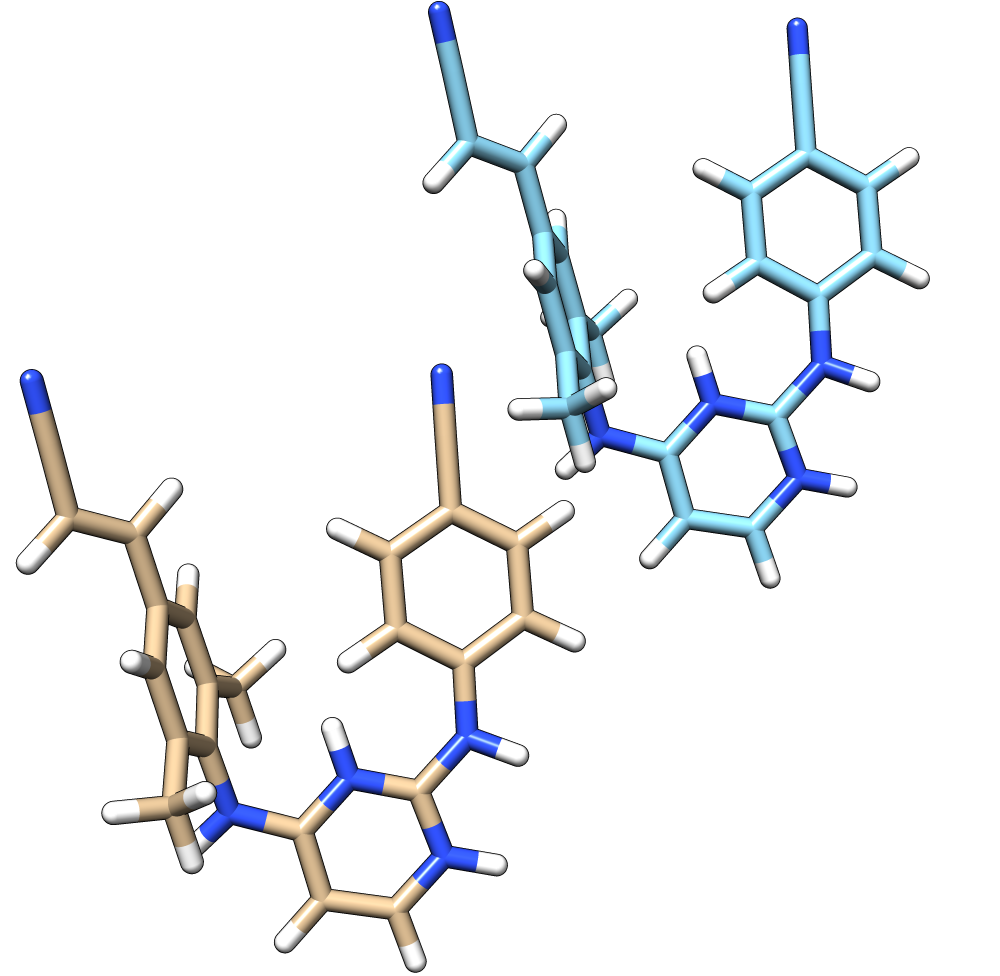
\includegraphics[width=0.32\linewidth]{PositionalDOF.png}
}
\subfloat[Orientational degree of freedom.]
{
  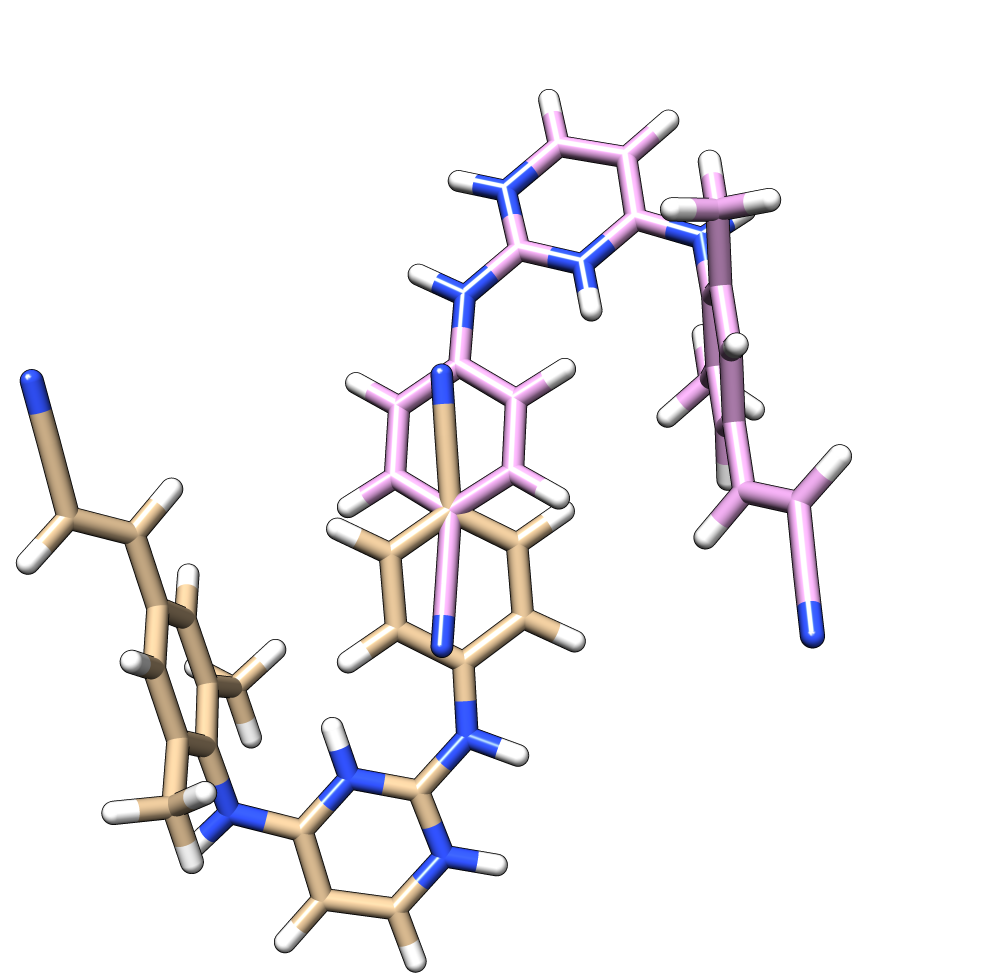
\includegraphics[width=0.32\linewidth]{OrientationalDOF.png}
}
\subfloat[Torsional degree of freedom.]
{
  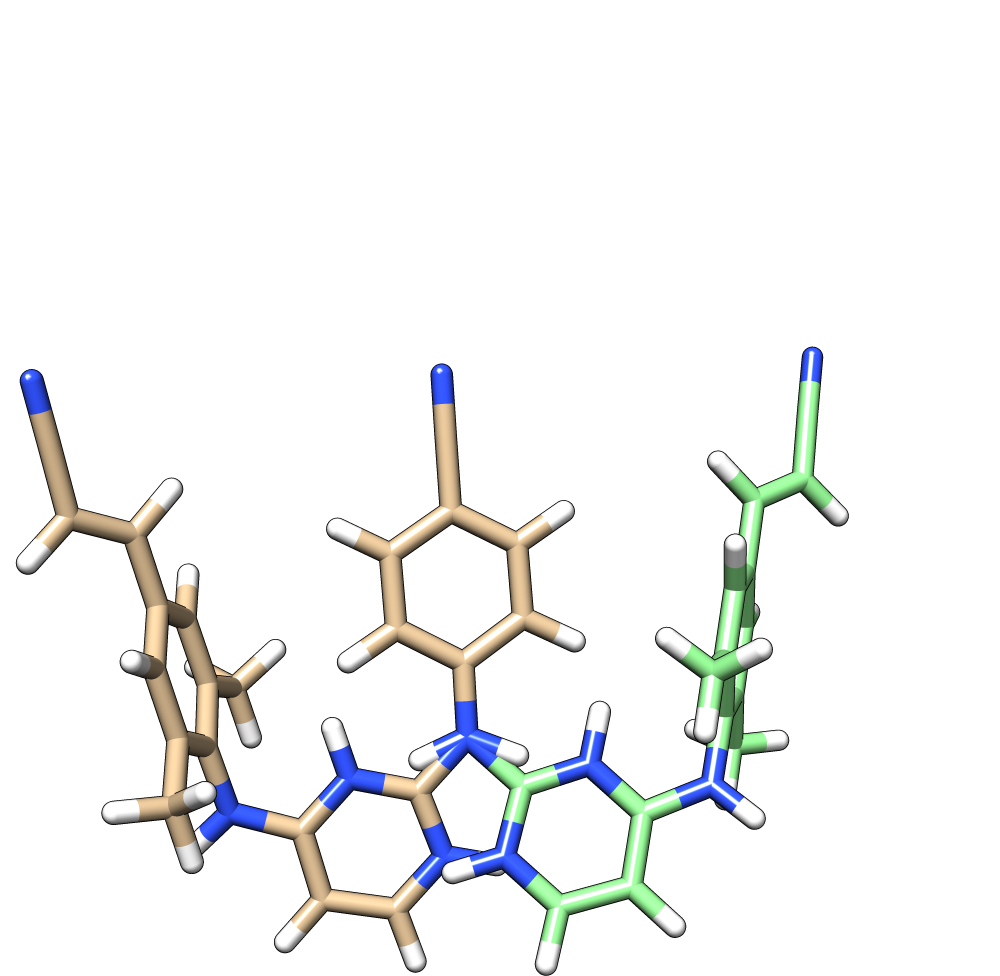
\includegraphics[width=0.32\linewidth]{TorsionalDOF.png}
}
\caption{Positional, orientational and torsional degree of freedom.}
\label{background:DegreeOfFreedom}
\end{figure*}

Treating a docking program as a black box, its input includes the 3D structures of a protein and a ligand, while its output includes several predicted conformations and their predicted binding affinity. For the protein input, thanks to the rapid evolution of X-ray crystallography and NMR (Nuclear Magnetic Resonance) technologies, more and more 3D structures of biological macromolecules at atomic level have been revealed and deposited into the world's largest repository PDB (Protein Data Bank) \citep{540,537}. As of 4 Sep 2012, there are 84,381 structures in PDB. For the ligand input, the ZINC database \citep{532,1178} contains over 21 million purchasable compounds in ready-to-dock, 3D formats. The TCM@Taiwan database \citep{528} is the world's largest and most comprehensive free down small molecular database on traditional Chinese medicine. In addition, the PubChem database \citep{526} is a public repository for biological properties of small molecules, containing biological test results for more than 700,000 compounds. The PDBbind database \citep{529,530} and the CSAR NRC HiQ Set \citep{857,960} are collections of binding affinities for protein-ligand complexes with known 3D structures. The refined set of PDBbind v2011 and the two sets of CSAR NRC HiQ Set 24Sept2010 comprise 2,455 and 343 protein-ligand complexes respectively, with experimentally determined binding affinity data. For the output, PyMOL \citep{1221}, Chimera \citep{1219}, VMD \citep{1220}, AutoDockTools4 \citep{596}, ViewDock TDW \citep{559}, PoseView \citep{748} and LigPlot+ \citep{951} can be used to visualize docked conformations and plot putative interaction charts. AuPosSOM \citep{598} can be used to cluster docked conformations. BEDROC \citep{490} and SLR \citep{489} can be used as statistical metrics for docking method evaluation.

Treating a docking program as a white box, it consists of two typical components, an algorithm to explore the conformational space of the ligand and the protein, and a scoring function to predict binding affinity given a conformation. Over recent decades, dozens of docking programs have been developed, such as DOCK \citep{1222}, AutoDock 4 \citep{785,596}, AutoDock Vina \citep{595}, QuickVina \citep{1193}, PLANTS \citep{610,607,779}, FITTED \citep{602}, CDOCK \citep{1224}, and CRDOCK \citep{1200}. Likewise, dozens of scoring functions have also been developed, such as RF-Score \citep{564}, SFCscore \citep{581}, LISA \citep{775}, and NNScore 2.0 \citep{977}. Refer to survey papers for a more complete list \citep{493,922} and for program comparison \citep{556,637}.

Amongst a sea of docking programs, AutoDock Vina \citep{595} (hereafter Vina for short) is a competitive one. It is free and open source under Apache License 2.0. It has been shown to run faster than its predecessor AutoDock 4 \citep{596} by an order of magnitude when benchmarking on virtual screening for HIV protease inhibitors \citep{556}. Released in the second half of 2010, Vina has been cited over 400 times and adopted by a wide community of researchers. Indeed, it is intensively used in our research projects too. In Vina, the binding affinity is evaluated as free energy. The lower the free energy, the higher the binding affinity. There is a PyMOL plugin for AutoDock and Vina \citep{609}. MOLA is a bootable, self-configuring system for virtual screening using AutoDock4/Vina on computer clusters \citep{773}. VSDK is a console application system of virtual screening of small molecules using AutoDock Vina on Windows \citep{1268}. AUDocker LE is a GUI for virtual screening with AutoDock Vina on Windows \citep{1250}.

In addition to pure docking program development, there is also a pool of successful case studies of using protein-ligand docking programs to discover novel and potent ligands for pharmacological proteins of therapeutic interest. To name a few, Vina was used for docking studies on the HEPT derivatives of HIV-1 reverse transcriptase \citep{843}, for side-chain residue flexibility study of VEGFR-2 (Vascular Endothelial Growth Factor Receptor 2), a known protein target for anti-angiogenic agents \citep{1084}, for identification of novel inhibitors of sirtuin 2, a NAD\textsuperscript{+}-dependent histone deacetylase enzyme \citep{1177}, and for repurposing study of FDA-approved drugs for cancer therapy in order to screen for compounds that potentially inhibit MDM2, an E3 ubiquitin ligase that polyubiquitinates p53 \citep{1230}. Such exciting success stories prove the real power of protein-ligand docking for computer-aided drug discovery.

Protein-ligand docking predicts the preferred conformation and binding affinity of a small ligand when it is non-covalently bound to a specific binding site of a macro protein. Up to date, there are hundreds of docking programs \citep{493,922}. The AutoDock series is the most cited docking software in the research community. AutoDock has contributed to the discovery of several drugs, including the first clinically approved HIV integrase inhibitor \citep{1169}. Technically speaking, AutoDock is single threaded \textit{per se}. Following its initial release, several parallel implementations were developed, using either multithreading or computer cluster \citep{115,560,782}.

In 2009, AutoDock Vina \citep{595} was released. As the successor of AutoDock 4 \citep{596}, AutoDock Vina significantly improves the average accuracy of the binding mode predictions while running two orders of magnitude faster with multithreading \citep{595}. It was compared to AutoDock 4 on selecting active compounds against HIV protease, and was recommended for docking large molecules \citep{556}. Its functionality of semi-flexible protein docking by enabling flexibility of side-chain residues was evaluated on VEGFR-2 \citep{1084}. To further facilitate the usage of AutoDock Vina, auxiliary tools were subsequently developed, including a PyMOL plugin for program settings and visualization \citep{609}, and a bootable operating system for computer clusters \citep{773}. AutoDock Vina is free and open source under Apache License 2.0. So far it has been cited by over 400 publications according to Google Scholar, making it a very competitive docking program.

In 2011, inspired by AutoDock Vina, we developed idock 1.0 \citep{1153}, a multithreaded virtual screening tool for flexible ligand docking. idock inherits from AutoDock Vina the accurate scoring function and the efficient optimization algorithm, and meanwhile introduces a fruitful of innovations, such as receptor and grid map caching for large-scale virtual screening, revised numerical model for much faster approximation, capability of automatic detection and deactivation of inactive torsions, utilization of our lightweight thread pool to parallelize grid map creation and reuse threads, utilization of the new C++11 feature of rvalue references to avoid frequent memory reallocation, and accelerated parsers for both receptor and ligand. When benchmarked on docking 10,928 drug-like ligands against HIV reverse transcriptase, idock 1.0 achieved a speedup of 3.3 in terms of CPU time and a speedup of 7.5 in terms of elapsed time on average compared to AutoDock Vina.

\section{Methods}

\subsectino{PDBQT specification}

\begin{figure}
\centering
%\includegraphics[width=\textwidth]{../idock/OutputPDBQT.png}
\caption{Verbose output of idock in PDBQT format.}
\label{idock:OutputPDBQT}
\end{figure}

Figure \ref{idock:Flowchart} shows the overall flowchart of idock. During initialization, idock precalculates the scoring function for all possible combinations of atom type pairs and interatomic distances. It parses the receptor and determines the atom types with the aid of residue sequence, and creates a thread pool to hold reusable threads. Then it enters a loop and fetches a ligand from a user-specified input folder to perform docking. It parses the ligand and determines the atom types with the aid of branch information, and meanwhile automatically detects and deactivates inactive torsions. It builds grid maps of granularity 0.15625 \AA\ by default on the fly by multithreading, and distributes multiple independent Monte Carlo tasks to the thread pool for concurrent execution. Then it merges the conformations from separate threads and clusters them with RMSD 2.0 \AA, and dumps them to the user-specified output folder and displays the predicted free energy on screen. It proceeds with the next ligand automatically until all are docked. Finally it destroys the thread pool and releases memory resources.

\begin{figure}
\centering
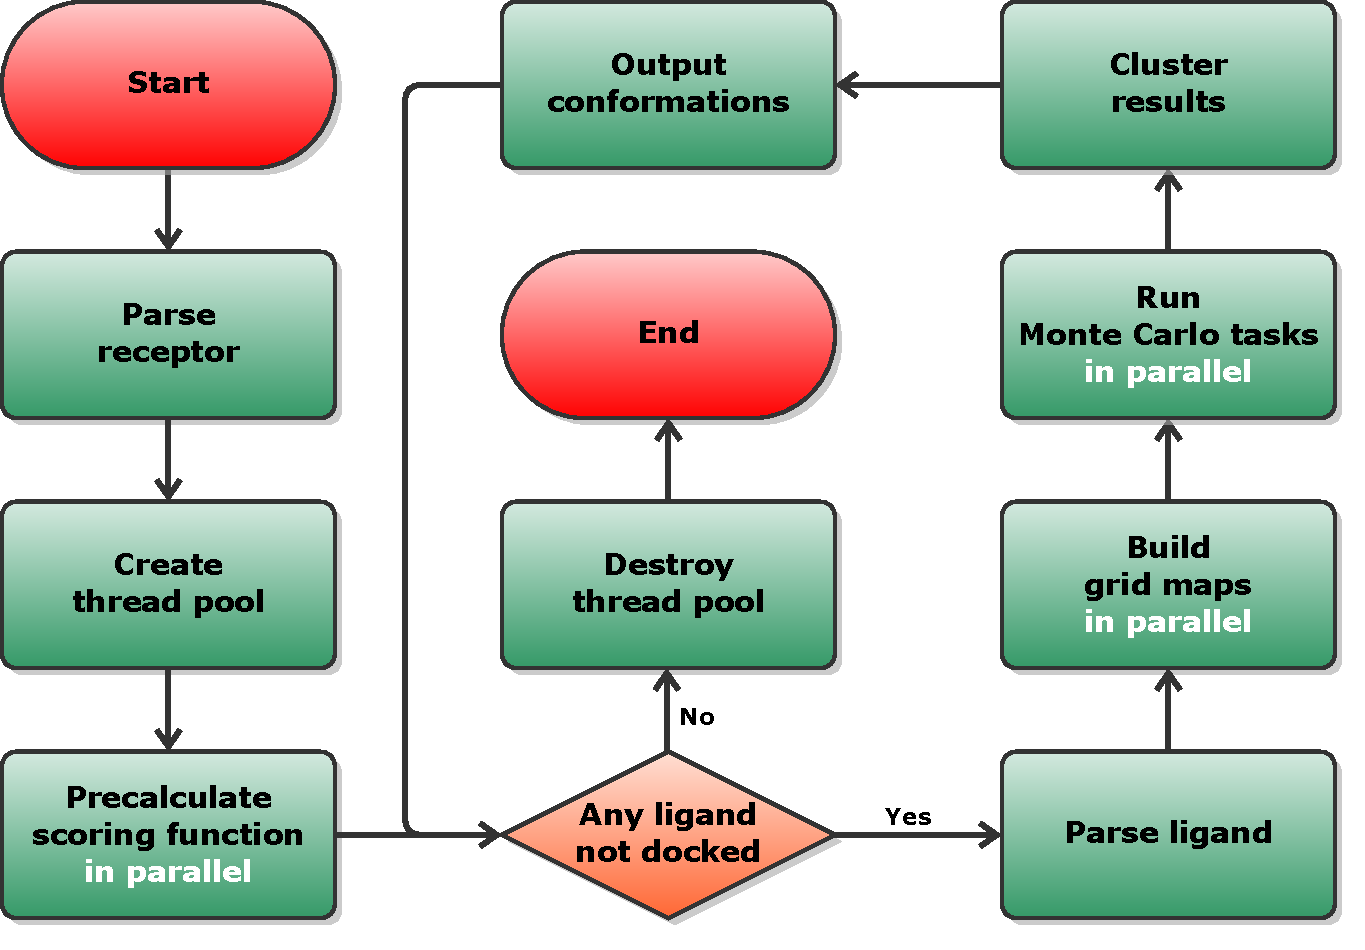
\includegraphics[width=\linewidth]{../idock/Flowchart.pdf}
\caption{Flowchart of idock.}
\label{idock:Flowchart}
\end{figure}

\subsection{Scoring Function}

Both idock and Vina share exactly the same scoring function, which is made up of a conformation-dependent part and a conformation-independent part. The conformation-dependent part is a weighted sum of five terms over all the pairs of atom $i$ and atom $j$ that can move relative to each other. It is calculated from equations \eqref{eqn:e} and \eqref{eqn:eij} where $t_i$ and $t_j$ are the atom types of $i$ and $j$ respectively, and $r_{ij}$ is their interatomic distance. The five terms are calculated from equations \eqref{eqn:Gauss1} to \eqref{eqn:HBonding} where $d_{ij}$ is the surface distance calculated from equation \eqref{eqn:dij} where $R_{t_i}$ and $R_{t_j}$ are the Van der Waals radii of $t_i$ and $t_j$ respectively (Figure \ref{idock:Distance}). All the units are in \AA. The weighting coefficients and the cut off at $r_{ij}$ = 8 \AA\ of the five terms are borrowed from Vina. The optimization algorithm attempts to find the global minimum of $e$ and other low-scoring conformations, which it then ranks.
\begin{equation}
\label{eqn:e}
e = \sum_{i < j} e_{ij}
\end{equation}
\begin{eqnarray}
\label{eqn:eij}
e_{ij} &=& (-0.035579) * Gauss_1(t_i, t_j, r_{ij}) \nonumber \\
       &+& (-0.005156) * Gauss_2(t_i, t_j, r_{ij}) \nonumber \\
       &+& (+0.840245) * Repulsion(t_i, t_j, r_{ij}) \nonumber \\
       &+& (-0.035069) * Hydrophobic(t_i, t_j, r_{ij}) \nonumber \\
       &+& (-0.587439) * HBonding(t_i, t_j, r_{ij})
\end{eqnarray}
\begin{equation}
\label{eqn:Gauss1}
Gauss_1(t_i, t_j, r_{ij}) = e^{-(d_{ij} / 0.5)^2}
\end{equation}
\begin{equation}
\label{eqn:Gauss2}
Gauss_2(t_i, t_j, r_{ij}) = e^{-((d_{ij} - 3) / 2)^2}
\end{equation}
\begin{equation}
\label{eqn:Repulsion}
Repulsion(t_i, t_j, r_{ij}) =
\begin{cases}
d_{ij}^2 & \text{if } d_{ij} < 0\\
0 &\text{if } d_{ij} \geq 0
\end{cases}
\end{equation}
\begin{equation}
\label{eqn:Hydrophobic}
Hydrophobic(t_i, t_j, r_{ij}) =
\begin{cases}
1 & \text{if } d_{ij} \leq 0.5\\
1.5 - d_{ij} & \text{if } 0.5 < d_{ij} < 1.5\\
0 & \text{if } d_{ij} \geq 1.5\\
\end{cases}
\end{equation}
\begin{equation}
\label{eqn:HBonding}
HBonding(t_i, t_j, r_{ij}) =
\begin{cases}
1 & \text{if } d_{ij} \leq -0.7\\
d_{ij} / (-0.7) & \text{if } -0.7 < d_{ij} < 0\\
0 & \text{if } d_{ij} \geq 0\\
\end{cases}
\end{equation}
\begin{equation}
\label{eqn:dij}
d_{ij} = r_{ij} - (R_{t_i} + R_{t_j})
\end{equation}
\begin{figure}
\centering
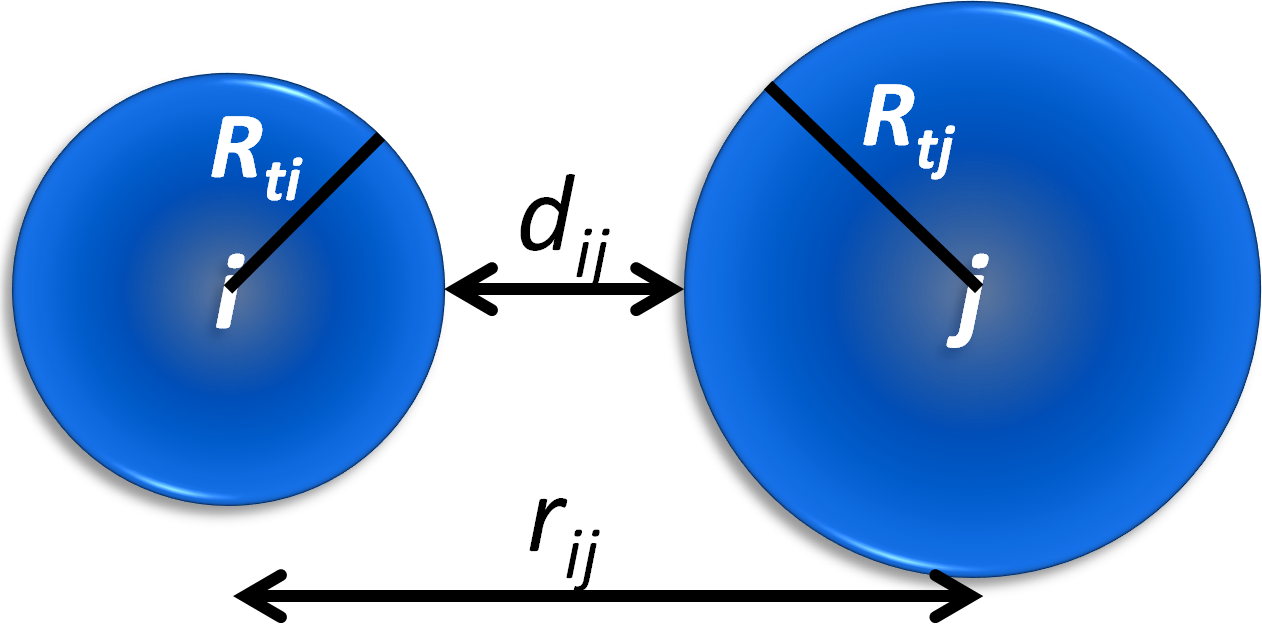
\includegraphics[width=\linewidth]{../idock/Distance.png}
\caption{Relationship between surface distance $d_{ij}$ and interatomic distance $r_{ij}$.}
\label{idock:Distance}
\end{figure}
The conformation-dependent part can be seen as the sum of intermolecular and intramolecular contributions. Hence equation \eqref{eqn:e} can be rewritten into equation \eqref{eqn:inter-intra} where $e_{inter}$ is the summation over all the heavy atoms between receptor and ligand, and $e_{intra}$ is the summation over all the 1-4 ligand heavy atoms that are separated by three consecutive covalent bonds and can move relative to each other.
\begin{equation}
\label{eqn:inter-intra}
e = e_{inter} + e_{intra}
\end{equation}
The conformation-independent part penalizes $e_{inter}$ for ligand flexibility. The predicted free energy of the $k$th conformation for output, denoted as $e'_k$, is calculated from equation \eqref{eqn:FlexibilityPenalty} where $k$ is the subscript for conformation, $e_k$ is the conformation-dependent score of the $k$th conformation calculated from equation \eqref{eqn:e}, $e_{intra,1}$ is the $e_{intra}$ of the first, i.e. lowest-scoring conformation, $N_{ActTors}$ is the number of active torsions and $N_{InactTors}$ is the number of inactive torsions of the ligand. Note that $e_{intra,1}$, rather than $e_{intra,k}$, acts as subtrahend in order to preserve the ranking.
\begin{equation}
\label{eqn:FlexibilityPenalty}
e'_k = \frac{e_k - e_{intra,1}}{1 + 0.05846 * (N_{ActTors} + 0.5 * N_{InactTors})}
\end{equation}
The value of $e_{ij}$ is basically a function of three variables, namely $t_i$, $t_j$, and $r_{ij}$. These three variables have both a known lower bound and a known upper bound, so it is possible to precalculate the scoring function. Since there are 17 atom types implemented in idock, the pair of $t_i$ and $t_j$ can have 153 (=17*18/2) different combinations. Since $r_{ij}$ is cut off at 8 \AA, idock uniformly samples 16,384 points in range [0, 8] to turn the continuous domain into a concrete domain, resulting in an average absolute error of merely 0.002 kcal/mol. During program initialization, idock precalculates $e_{ij}$ from equation \eqref{eqn:eij} for 153*16384 possible combinations of $t_i$, $t_j$, and $r_{ij}$. During optimization, idock approximates the true value of $e_{ij}$ by direct assignment rather than linear interpolation for faster evaluation of $e_{ij}$ at the cost of a little bit longer precalculation time and a bit more memory storage.

\subsection{Grid Maps}

In order to fast evaluate $e_{inter}$, grid maps are often built. A grid map of atom type \textit{t} is constructed by placing virtual probe atoms of atom type \textit{t} along the X, Y, Z dimensions of the search box at a certain granularity (Figure \ref{idock:GridMap}). The $e_{inter}$ value of these probe atoms are precalculated, so the $e_{inter}$ value of a ligand heavy atom can be approximated in some way. In Vina, the grid map granularity is hard coded to be 0.375 \AA, and the approximation is done by linear interpolation of the 8 corner probe atoms of the residing subbox. This kind of interpolation involves reading of 8 $e_{inter}$ values, computation of 3 $\alpha$ values, 12 floating-point subtractions, 24 floating-point multiplications, and 7 floating-point additions, which turned out to be a performance bottleneck when we profiled Vina. In contrast, idock exposes grid map granularity as an optional program argument with a tuned default value of 0.15625 \AA. Likewise, due to a higher density of probe atoms, idock substitutes direct assignment for linear interpolation for much faster evaluation of $e_{inter}$ at the cost of longer precalculation time and larger memory storage. Therefore, the creation of grid maps is carried out on the fly only when necessary and abstracted into parallel tasks, which are then distributed to the thread pool for concurrent execution.

\begin{figure}
\centering
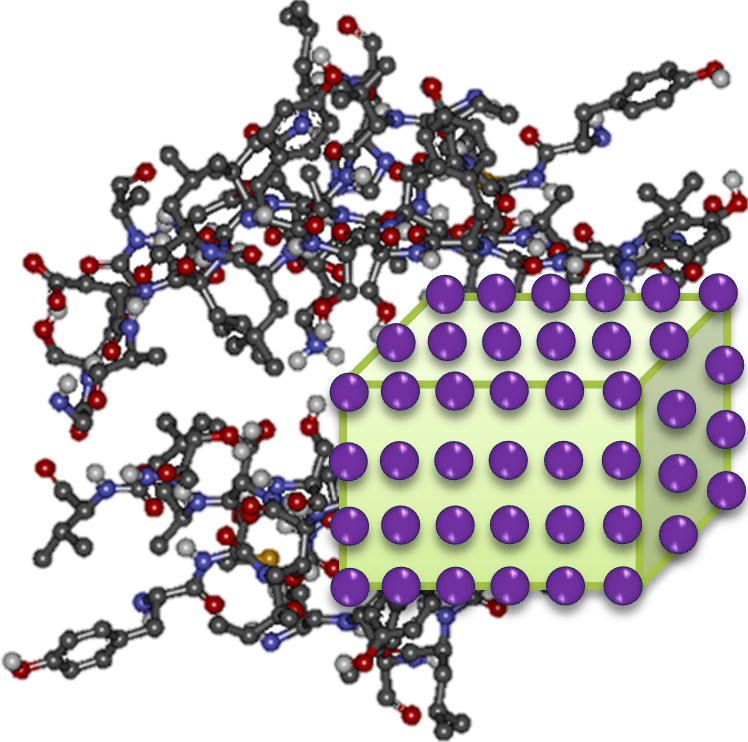
\includegraphics[width=\linewidth]{../idock/GridMap.png}
\caption{Grid map for fast evaluation of $e_{inter}$. Probe atoms are shown in purple.}
\label{idock:GridMap}
\end{figure}

\subsection{Optimization Algorithm}

Both idock and Vina use Monte Carlo algorithm for global optimization and Broyden-Fletcher-Goldfarb-Shanno (BFGS) \cite{786} Quasi-Newton method for local optimization. A succession of steps consisting of a mutation and a BFGS local optimization are taken, with each step being accepted according to the Metropolis criterion (Figure \ref{idock:MonteCarlo}, modified from \cite{493}). These steps are repeated over \textit{N} iterations, where \textit{N} correlates to the complexity of the ligand regarding number of heavy atoms and number of torsions. BFGS approximates the inverse Hessian matrix of the scoring function. It uses not only the value of the scoring function but also its gradient, which are the derivatives of the scoring function with respect to the position and orientation of the ligand, and the torsions for the active rotatable bonds in the ligand. A BFGS iteration derives a descent direction from the approximate inverse Hessian matrix, derives a step length along the descent direction by line search, and updates the approximation of inverse Hessian matrix. Both programs achieve multithreading by concurrently running multiple independent Monte Carlo tasks starting from random initial conformations.

Though both programs share similar optimization algorithms, their implementations differ. Compared with Vina, the Monte Carlo iterations in idock are far fewer and the BFGS iterations are more. On one hand, the fewer number of Monte Carlo iterations is compensated by a larger number of parallel Monte Carlo tasks, which is 64 by default in idock compared to 8 in Vina, guaranteeing better conformational diversity and higher CPU utilization on multi-core computers. On the other hand, the stopping criterion of BFGS local optimization does not depend on an estimated number of iterations, which is the case in Vina, but depends on the outcome of line search. The BFGS local optimization stops if and only if no appropriate step length can be obtained by line search, thus increasing the probability of finding optimal local minimums.

\subsection{Native Support of Virtual Screening}

Vina is optimized for single-ligand docking rather than virtual screening. When it comes to docking a large pool of ligands, Vina has to be invoked multiple times, repeatly parsing the same receptor and creating the same grid maps, thus degrading performance.

idock supports virtual screening in a native manner. It docks a directory of ligands instead of a single ligand, and reuses receptor and grid maps (Note the loop in the flowchart). Given a very large amount of ligands to dock, idock indirectly supports two-phase virtual screening via two consecutive runs. In the first run, idock performs coarse but fast virtual screening without writing any conformations to file, aiming to quickly shortlist a few candidate compounds. In the second run, idock performs fine but slow virtual screening with a significantly larger number of Monte Carlo tasks per ligand, writing as many conformations to file as possible and aiming to refine the predicted free energy as well as predicted conformation of candidate compounds. Such a 2-phase docking methodology can remarkably reduce overall execution time while avoiding the risk of filtering out potentially promising compounds, controlling the false negative rate at an acceptable level.

\subsection{Detection of Inactive Torsions}

idock automatically detects and deactivates inactive torsions, which are presented and activated in the input file in pdbqt format but have no impact on the overall scoring, such as \textemdash{OH} and \textemdash{NH$_2$}, because they only rotate the hydrogens. Figure \ref{idock:InactiveTorsions} shows an example ligand which contains 4 active torsions defined by the python script \textit{prepare\_ligand4.py} provided by AutoDock Tools \cite{785,596}. Two of them, highlighted in yellow, only rotate hydrogens and thus have no contributions to the scoring. They are re-classified as inactive torsions and deactivated while being parsed in idock. This kind of automatic detection and deactivation of inactive torsions reduces the torsional degrees of freedom to optimize in the local optimization step, leading to easier finding of local minimums.

\begin{figure}
\centering
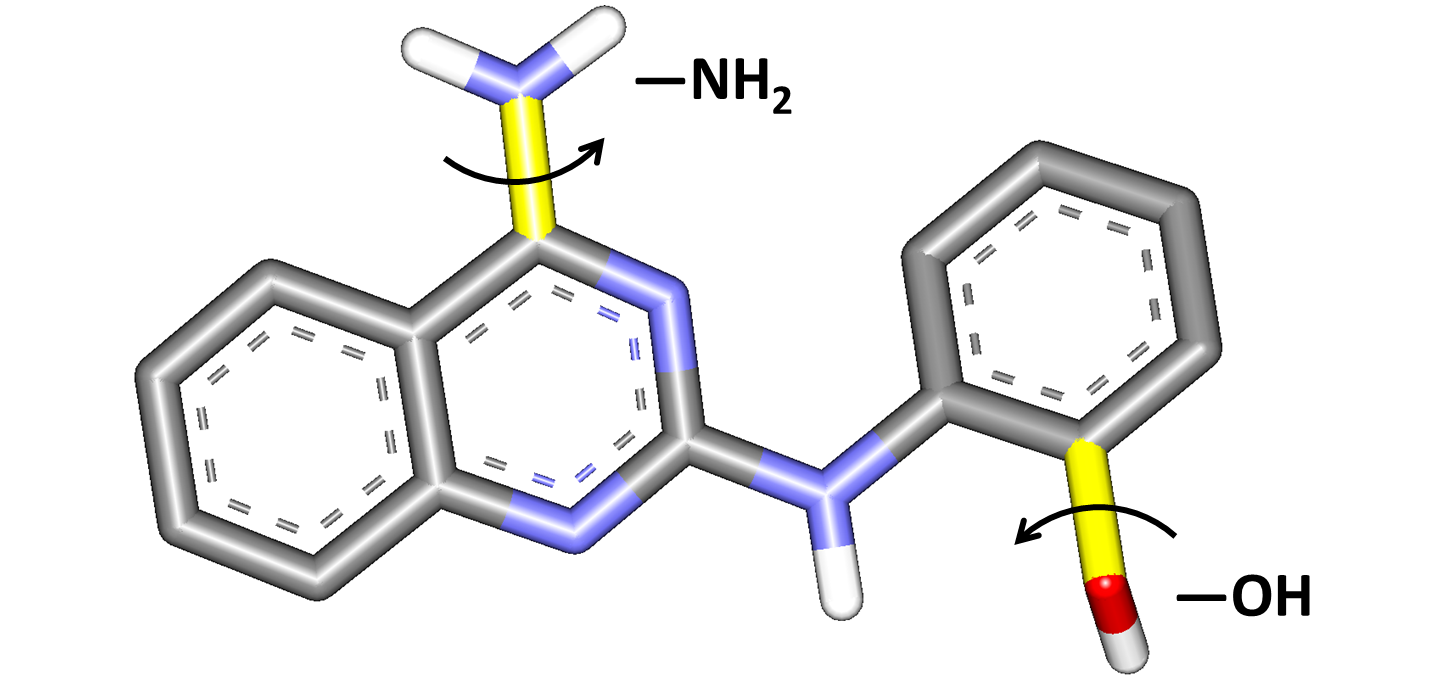
\includegraphics[width=\linewidth]{../idock/InactiveTorsions.png}
\caption{Example of inactive torsions highlighted in yellow. Nonpolar hydrogens are not shown for clarity.}
\label{idock:InactiveTorsions}
\end{figure}

\subsection{Miscellaneous Improvements}

idock implements a lightweight thread pool in order to reuse threads and maintain a high CPU utilization throughout the entire screening procedure. During program initialization, idock creates a thread pool of $N$ threads, where $N$ is the number of CPU cores automatically detected, or can be specified by user via a command line argument. When idle, the threads sleep. When tasks arrive, the threads compete for tasks. The thread that completes its current task will automatically fetch a pending one to execute until all are done. Synchronization is implemented to ensure the full completeness of tasks and availability of results. The task here is an abstract concept in programming sense and can be instantiated either as scoring function tasks, grid map tasks or Monte Carlo tasks. To be exact, the thread pool in fact parallelizes the precalculation of scoring function, the creation of grid maps, and the execution of Monte Carlo tasks.

idock enables automatic recovery. While docking is in progress, in case the process gets killed accidentally and restarted some time later, idock not only resumes docking from the previous stopping point, skipping ligands that were already docked in a previous run, but also detects and reports possible file content errors, ensuring all the output ligands are well written.

idock supports reading and writing compressed ligand files with in gzip/bzip2 format, resulting in a file footprint as low as just one eighth of the raw size using gzip (Figure \ref{idock:Compression}). This new functionality turns out to be extremely handy given an enormous amount of ligands to dock.

Both idock and Vina support 16 common chemical elements, which are H (hydrogen), C (carbon), N (nitrogen), O (oxygen), F (fluorine), Mg (magnesium), P (phosphorus), S (sulfur), Cl (chlorine), Ca (calcium), Mn (manganese), Fe (iron), Zn (zinc), Se (selenium), Br (bromine), and I (iodine). idock adds 9 additional elements, which are Na (sodium), K (potassium), Co (cobalt), Ni (nickel), Cu (copper), Sr (strontium), Cd (cadmium), Hg (mercury), and As (arsenic). Hence idock supports as many as 25 chemical elements, covering the majority of ligand atom types (Figure \ref{idock:ChemicalElements}). % Untested feature

idock outputs verbose information to docked PDBQT files, including total free energy normalized by torsional degree of freedom (Equation \eqref{eqn:FlexibilityPenalty}), total free energy, inter-ligand free energy, intra-ligand free energy, putative hydrogen bonds, and per-atom inter-ligand free energy (Figure \ref{idock:OutputPDBQT}). The normalized total free energy is used in ligand ranking. The output of total free energy, inter-ligand free energy and intra-ligand free energy provides an alternative ranking option using derived efficiency indexes \citep{335,336,337}. The per-atom inter-ligand free energy facilitates interaction hotspot determination, and helps improving potency by altering certain chemical moieties while retaining those critical for binding.

idock extracts the above records from docked PDBQT files, sorts them in the ascending order of normalized total free energy, and writes them to a CSV (Comma-Separated Vector) file for subsequent analysis (Figure \ref{idock:OutputCSV}). Users can derive their own efficiency indexes \citep{335,336,337} and re-sort the records for their particular applications.

idock implements our own lightweight thread-safe progress bar, reporting progress every 10\% Monte Carlo tasks per ligand. idock better supports rvalue references and move semantics in C++11 to boost performance. idock flattens the tree-like recursive data structure of ligand as used in AutoDock Vina into simple linear array structure to ensure a high data cache hit rate and easy coding. idock accelerates the assignment of atom types by making use of residue information for receptor and branch information for ligand.

\section{Benchmarks and Results}

idock x86\_64 v1.5 and AutoDock Vina x86 v1.1.2 were evaluated on desktop computers with Intel Core i5-2400 CPU @ 3.10GHz and 4GB DDR3 RAM under Mac OS X 10.7.4 Build 11E53. Arguments to both programs were left as default. By default, both programs output 9 predicted conformations per ligand. The benchmarks include comparison of their redocking performance in terms of predicted conformations, and comparison of their virtual screening performance in terms of execution time, memory usage, predicted free energy, and predicted conformations.

\section{Discussion and Conclusion}

We have developed idock for protein-ligand docking, inheriting from Vina the accurate scoring function and the efficient optimization algorithm, and meanwhile introducing a fruitful of innovations in C++ implementations, data structures, numerical models, and Monte Carlo algorithms. idock implements its own thread pool to maintain a high CPU utilization throughout the entire screening procedure. It intensively utilizes modern C++11 techniques, particularly Rvalue references to avoid frequent reallocations of array data. It flattens Vina's tree-like recursive data structures into simple array structures to guarantee a high data cache hit rate. It automatically detects and deactivates inactive torsions and thus reduces the dimension of variables to optimize.

In Vina's official forum, there are tremendous requests for the support for virtual screening. The development of idock perfectly complements Vina. idock has built-in support for virtual screening. It searches for ligands in a user-specified folder and docks them one by one. It reuses threads and grid maps across multiple ligands. idock has very similar input and output arguments as Vina, so it should be quite easy for existing Vina users to transit to idock. Vina supports flexible receptor docking by rotating flexible side-chains. However, at the moment we have not yet implemented flexible receptor docking, which has been proved helpful in some cases \citep{1084}, so users who need this kind of docking should refer to Vina.

We performed large-scale protein-ligand docking with idock, and noticed that the high-rank ligands were usually those comparatively rigid ligands with few active torsions. Such phenomenon can be explained by equation \eqref{eqn:FlexibilityPenalty}. Fewer active torsions imply smaller denominator, or larger value in other words. We are considering replacing free energy by some ligand efficiency indexes \citep{335,336,337} for ranking.

\section{Availability}

idock is free and open source under Apache License 2.0. Precompiled executables for 32-bit and 64-bit Linux, Windows, Mac OS X, FreeBSD and Solaris, 13 docking examples, and a doxygen file for generating API documentations are available at https://github.com/HongjianLi/idock.

idock supports Linux and Windows, and can be easily extended to support Mac OS X, FreeBSD and Solaris. Accompanying with idock are 13 ready-to-use docking examples, a doxygen file for generating API documentations.

\chapterend
